\documentclass[aspectratio=169,10pt]{beamer}

\usetheme{Madrid}
\usecolortheme{default}
\setbeamertemplate{navigation symbols}{}
\setbeamertemplate{footline}[frame number]

\usepackage[utf8]{inputenc}
\usepackage[T1]{fontenc}
\usepackage{amsmath,amssymb,mathtools}
\usepackage{booktabs}
\usepackage{tikz}
\usepackage{xspace}
\usepackage{graphicx}
\usepackage{adjustbox}
\usepackage{natbib}
\usepackage{LogicYinfeng,StrategicYinfeng}
\usepackage{xcolor}
\setbeamercovered{transparent}

\definecolor{KRBlue}{RGB}{26,74,122}
\definecolor{KRTeal}{RGB}{0,120,115}
\definecolor{KRRust}{RGB}{156,78,42}
\definecolor{KRGray}{RGB}{70,75,80}

\setbeamercolor{title}{fg=KRBlue}
\setbeamercolor{frametitle}{fg=KRBlue}
\setbeamercolor{structure}{fg=KRTeal}
\setbeamercolor{block title}{bg=KRBlue!10,fg=KRBlue}
\setbeamercolor{block body}{bg=KRBlue!3,fg=black}
\setbeamercolor{alerted text}{fg=KRRust}

\newcommand{\WATL}{\ensuremath{\mathsf{WA{-}ATL}}\xspace}
\newcommand{\WCL}{\ensuremath{\mathsf{WA{-}CL}}\xspace}
\newcommand{\Benef}{\mathsf{Benef}}
\newcommand{\Danger}{\mathsf{Danger}}
\newcommand{\tr}{\mathit{tr}}
\newcommand{\SB}{\mathit{StrSB}}
\newcommand{\SH}{\mathit{StrSH}}

\title[Welfare-Affecting Capabilities]{Reasoning about Welfare-Affecting Capabilities in Concurrent Games}
\author[Y. Li and E. Lorini]{Yinfeng Li \and Emiliano Lorini}
\institute[IRIT]{IRIT, CNRS, University of Toulouse}
\date[KR 2026]{KR 2026}

\begin{document}

\begin{frame}
  \titlepage
\end{frame}

\begin{frame}{The Motivation}
  \begin{block}{Strategic ability is not only about achieving goals}
    In multi-agent systems, a coalition's choices may also affect the welfare of other agents.
  \end{block}

  \vspace{0.5em}
  \begin{columns}[T,onlytextwidth]
    \column{0.49\textwidth}
    \textbf{Classical ATL/CL asks}
    \begin{itemize}
      \item Can coalition $C$ ensure $\varphi$?
      \item Can $C$ keep $\varphi$ true forever?
    \end{itemize}

    \column{0.49\textwidth}
    \textbf{We also ask}
    \begin{itemize}
      \item Can $C$ benefit coalition $B$?
      \item Can $C$ harm coalition $H$?
      \item Can it do so while ensuring $\varphi$?
    \end{itemize}
  \end{columns}

  \vspace{0.6em}
  \centering
  \alert{Who is a potential benefactor, and who is a danger?}
\end{frame}

\begin{frame}{Conceptual Ingredients}
  \begin{columns}[T,onlytextwidth]
    \column{0.48\textwidth}
    \begin{block}{Harm and benefit}
      We adopt a consequentialist, non-comparative reading, where good and bad outcomes are represented through agents' preferences:
      \begin{itemize}
        \item harm: bringing about a bad outcome;
        \item benefit: bringing about a good outcome.
      \end{itemize}
      
    \end{block}

    \column{0.48\textwidth}
    \begin{block}{Danger}
      We follow a modal, non-probabilistic intuition for danger~\citep{Fassio2025OnDanger,Garland2003RiseOfRisk,Peschard2022PhilosophyRisk}:
      \begin{itemize}
        \item a coalition is dangerous if it has the potential to harm;
        \item potential means existence of a suitable strategy.
      \end{itemize}
    \end{block}
  \end{columns}

  \vspace{0.7em}
  \centering
  \large
  strategic capability~\citep{alur2002alternating,GorankoDrimmelenATL}\\
  +\\
  preference over outcomes~\citep{DBLP:conf/ifaamas/LiLM25}\\  
    $\quad \Downarrow \quad$\\
    welfare-affecting capability
\end{frame}

\begin{frame}{Main Contributions}
  \begin{enumerate}
    \item A semantics based on concurrent games enriched with agents' preferences over computations.
    \item New ATL and CL modalities for welfare-affecting strategic capabilities:
      \[
        \atlbh{C}{B}{H}\gamma
      \]
      ``$C$ has a strategy that benefits $B$, harms $H$, and guarantees $\gamma$.''
    \item Technical results:
      \begin{itemize}
        \item sound and complete axiomatization for the until-free fragment;
        \item polynomial embedding into standard ATL/CL with special atoms marking benefited and harmed agents;
        \item tight satisfiability complexity: \Exptime-complete for \WATL, \Pspace-complete for \WCL.
      \end{itemize}
  \end{enumerate}
\end{frame}

\begin{frame}{Models: Concurrent Games with Preferences}
  A model is a concurrent game model with regular preferences:
  \[
    M = \big(\St,\ACT,(\relAct{\jactatm})_{\jactatm\in\JACT},\preceq,\valProp\big).
  \]

  \begin{itemize}
    \item $\St$: non-empty set of states.
    \item $\ACT$: action names; $\JACT=\ACT^n$: action profiles.
    \item $\relAct{\jactatm}\subseteq \St\times \St$: transition relation for action profile $\jactatm$.
    \item for each agent $i$ and state $s$, a regular preference order
      \[
        \preceq_{i,s}
      \]
      over computations starting at $s$.
    \item $\valProp:\St\to 2^\ATM$: valuation function.
  \end{itemize}

  \begin{block}{Constraints for game structures}
    Collective choice determinism, independence of choices, and seriality.
  \end{block}
\end{frame}

\begin{frame}{Regularity of preferences}
  The preference order $\preceq_{i,s}$ is regular if it is a total preorder over computations starting at $s$ and:

  \begin{itemize}
    \onslide<1,4>{\item stable:\\
     for all computations $\lambda,\lambda'$ starting at $s$, if $\lambda(1)=\lambda'(1)$ and $\lambda\preceq_{i,s}\lambda'$, then $\lambda_{\geq 1}\preceq_{i,s'}\lambda'_{\geq 1}$, where $s'=\lambda(1)$;}
    \onslide<2,4>{\item well-founded:\\
    the worst computation exists;
    \item conversely well-founded:\\
    the best computation exists;}
    \onslide<3,4>{\item non-flat:\\
    there is $\lambda,\lambda'$ starting at $s$ such that $\lambda \prec_{i,s} \lambda'$.}
  \end{itemize}
\end{frame}

\begin{frame}{Running Example: Robots and Charging Rooms}
  \begin{columns}[T,onlytextwidth]
    \column{0.42\textwidth}
    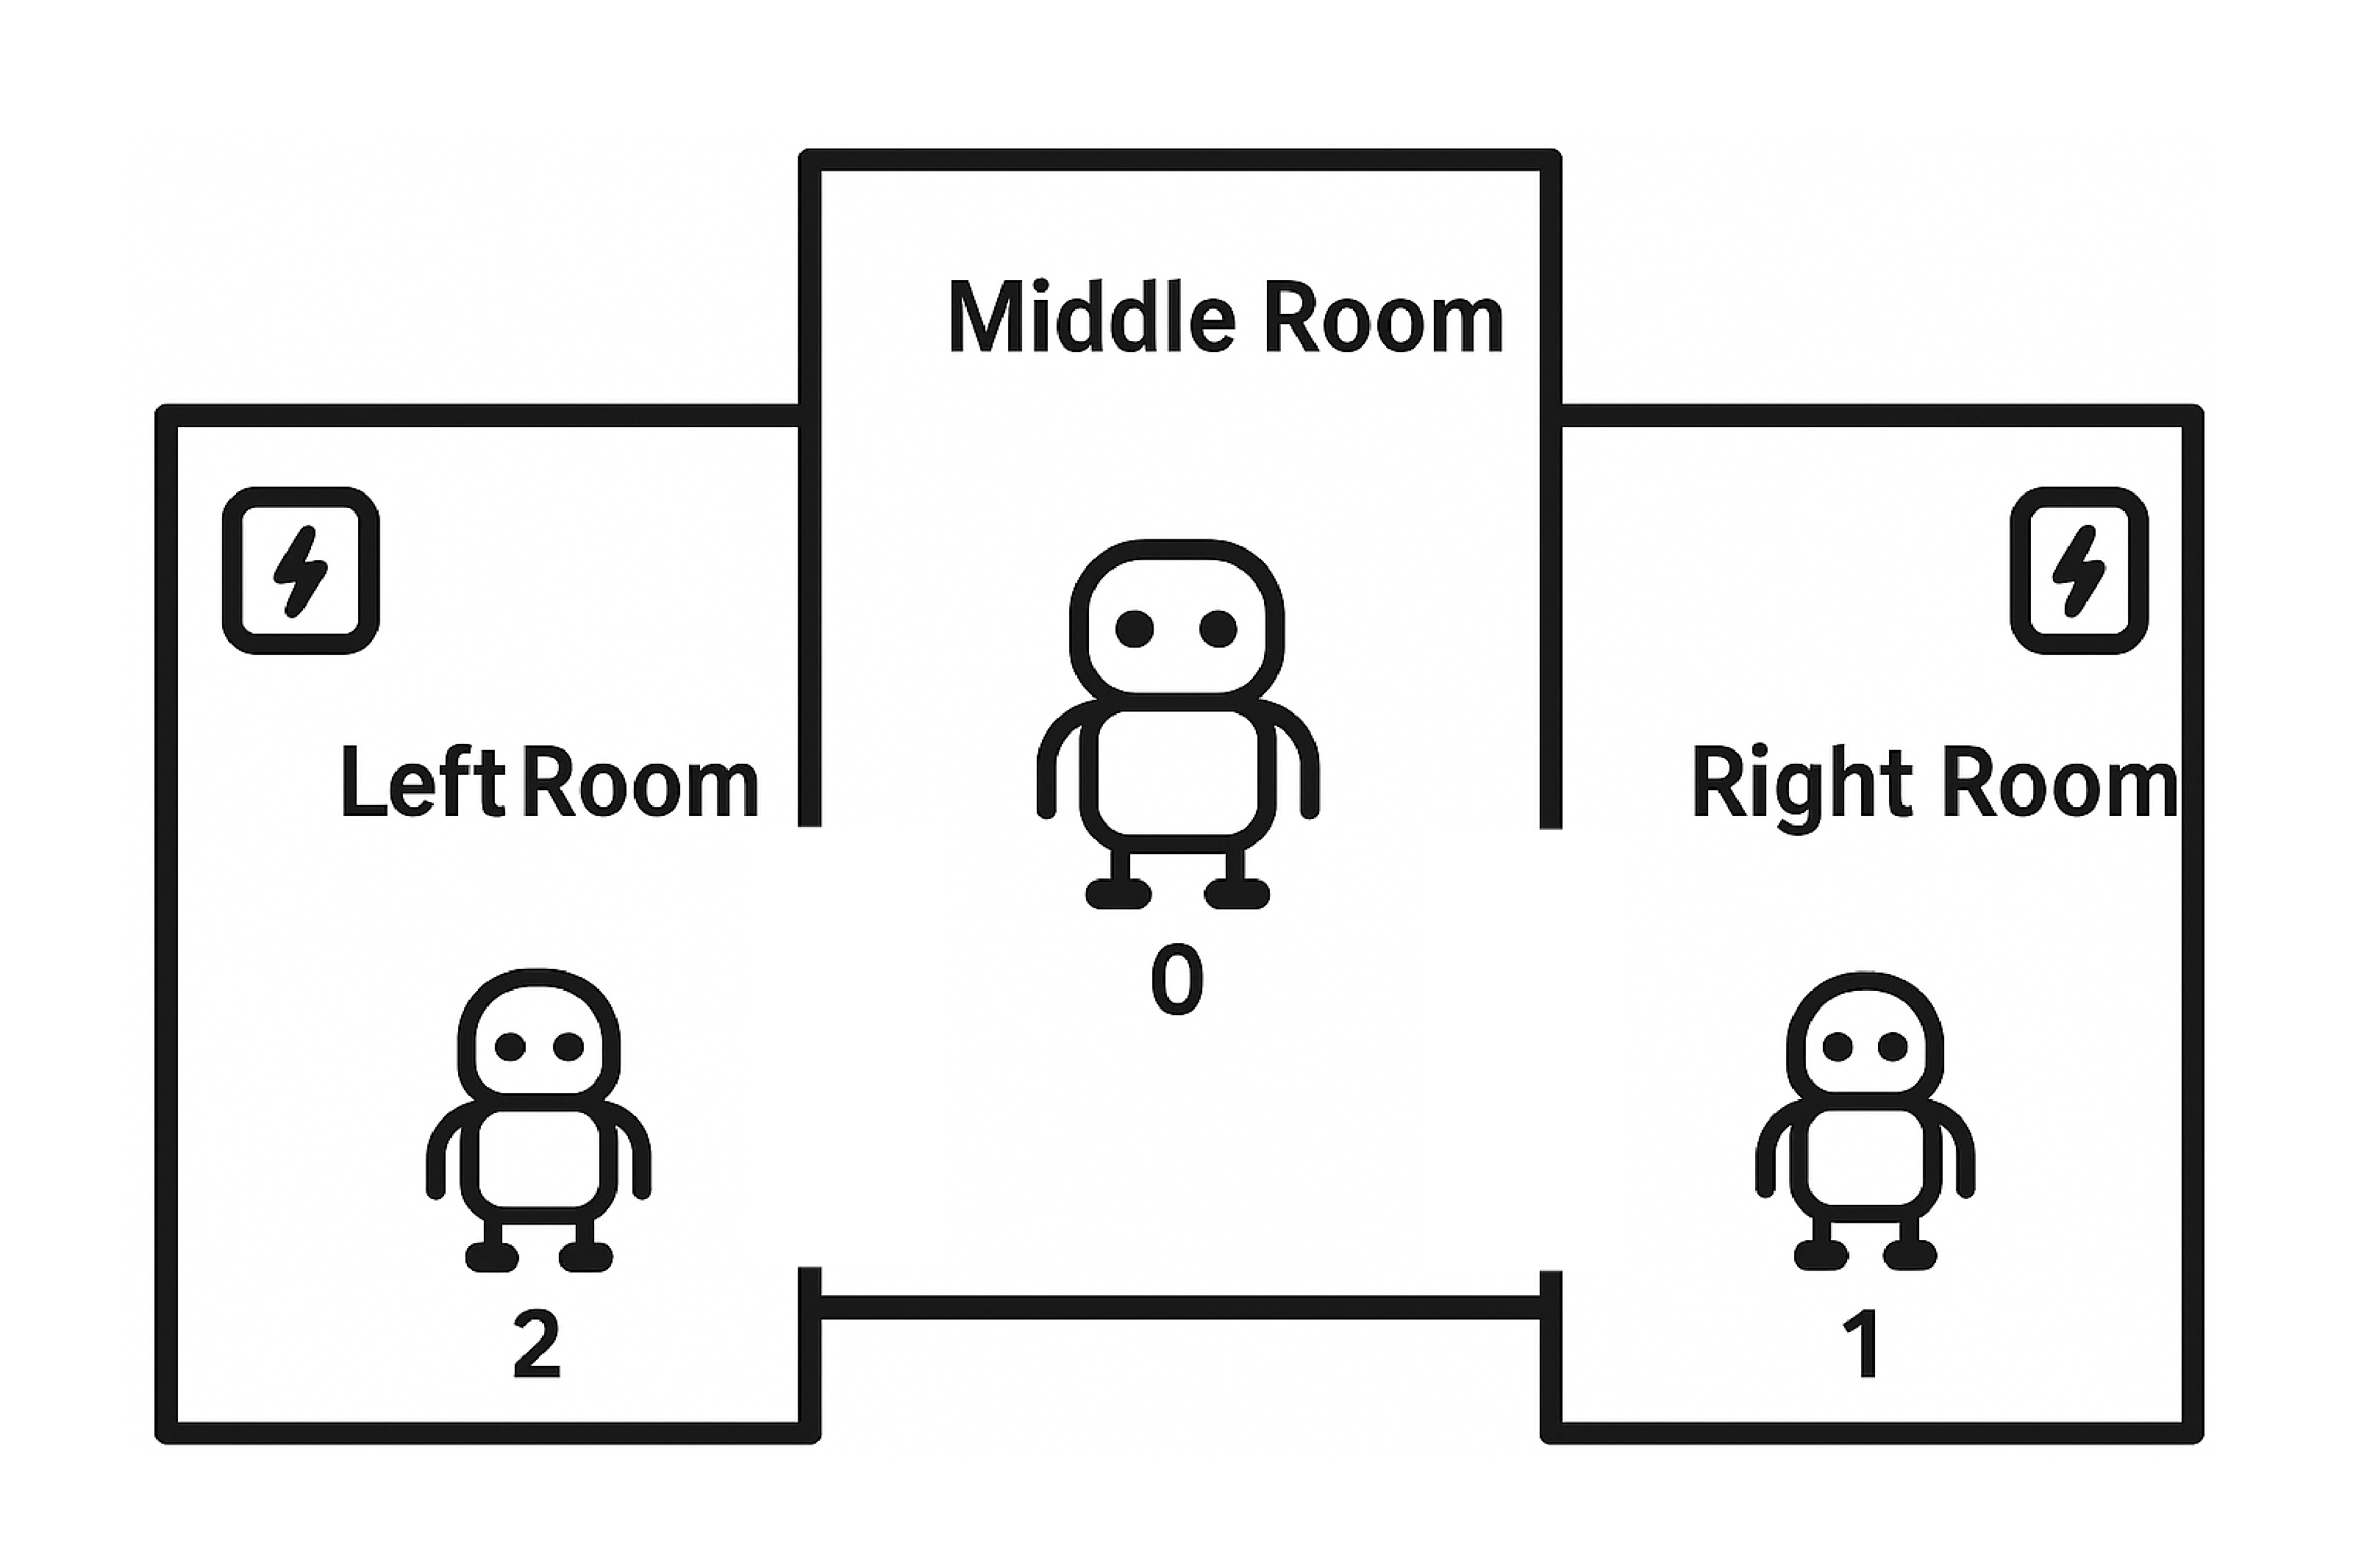
\includegraphics[width=\linewidth]{ImageSpace.pdf}

    \column{0.56\textwidth}
    \begin{itemize}
      \item Robot $0$ starts in the middle room.
      \item It wants to reach a charging station on the left or right.
      \item Robots $1$ and $2$ guard the right and left passages.
      \item Each guard can block or free its passage.
    \end{itemize}

    \vspace{0.4em}
    \begin{block}{Preference profile}
      Robot $0$ prefers computations where it eventually reaches a charging station.

      Robots $1$ and $2$ prefer computations where robot $0$ never reaches one.
    \end{block}
  \end{columns}
\end{frame}

\begin{frame}{Strong Benefit and Strong Harm}
  Let $\outset_\F(s,\js_C)$ be the computations compatible with strategy $\js_C$ from $s$.

  \vspace{0.3em}
  \begin{block}{Strongly beneficial for $B$}
    \[
      \js_C \in \SB^\Coalition_\M(s,B)
      \quad \text{iff} \quad
      \outset_\F(s,\js_C) \subseteq \Best_{i,s}
      \text{ for every } i\in B.
    \]
  \end{block}

  \begin{block}{Strongly harmful for $H$}
    \[
      \js_C \in \SH^\Coalition_\M(s,H)
      \quad \text{iff} \quad
      \outset_\F(s,\js_C) \subseteq \Worst_{i,s}
      \text{ for every } i\in H.
    \]
  \end{block}

  \vspace{0.2em}
  \centering
  Strong benefit/harm means guaranteeing best/worst outcomes for the affected coalition.
  \begin{block}{Fact}
    The coalition of robots $\{1,2\}$ has a strategy that is harmful to robot $0$ and beneficial to the guarding coalition.
  \end{block}
\end{frame}

\begin{frame}{The Language \WATL}
  \[
  \begin{array}{rcl}
    \varphi,\psi &::=& p \mid \neg\varphi \mid \varphi\wedge\psi
      \mid \atlbh{C}{B}{H}\gamma \\[0.2em]
    \gamma &::=& \X\varphi \mid \G\varphi \mid \varphi\U\psi
  \end{array}
  \]

  \vspace{0.6em}
  \begin{block}{Key modality}
    \[
      \atlbh{C}{B}{H}\gamma
    \]
    Coalition $C$ has a strategy which is beneficial for $B$, harmful to $H$, and guarantees temporal property $\gamma$.
  \end{block}

  \vspace{0.5em}
  Standard ATL is recovered as the special case:
  \[
    \atlop{C}\gamma \;\equiv\; \atlbh{C}{\emptyset}{\emptyset}\gamma.
  \]
\end{frame}

\begin{frame}{Semantics of the New Modality}
  \[
  (\M,s)\models \atlbh{C}{B}{H}\gamma
  \]
  iff there exists a strategy
  \[
    \js_C \in \SB^C_\M(s,B)\cap \SH^C_\M(s,H)
  \]
  such that every generated computation satisfies $\gamma$:
  \[
    \forall \lambda\in\outset_\F(s,\js_C),\quad
    (\M,\lambda)\models \gamma.
  \]

  \vspace{0.8em}
  \begin{block}{Three roles in one operator}
    \begin{itemize}
      \item $C$: the acting coalition;
      \item $B$: the coalition benefited by the strategy;
      \item $H$: the coalition harmed by the strategy.
    \end{itemize}
  \end{block}
\end{frame}

\begin{frame}{Potential Benefactor and Danger}
  The language gives compact definitions of the target notions.

  \vspace{0.8em}
  \begin{columns}[T,onlytextwidth]
    \column{0.48\textwidth}
    \begin{block}{Potential benefactor}
      \[
        \Benef(C,B)
        \;\equiv\;
        \atlbh{C}{B}{\emptyset}\X\top.
      \]
      Coalition $C$ has a strategy beneficial for $B$.
    \end{block}

    \column{0.48\textwidth}
    \begin{block}{Danger}
      \[
        \Danger(C,H)
        \;\equiv\;
        \atlbh{C}{\emptyset}{H}\X\top.
      \]
      Coalition $C$ has a strategy harmful to $H$.
    \end{block}
  \end{columns}

  \vspace{1em}
  In the robot model:
  \[
    (\M_{\mathit{rs}},s_0)\models
    \Benef(\{1,2\},\{1,2\}) \wedge \Danger(\{1,2\},\{0\}).
  \]
\end{frame}

\begin{frame}{Axiomatization}
  We axiomatize the until-free, or safety, fragment:
  \[
  \varphi ::= p \mid \neg\varphi \mid \varphi\wedge\varphi
  \mid \atlbh{C}{B}{H}\X\varphi
  \mid \atlbh{C}{B}{H}\G\varphi.
  \]

  \vspace{0.5em}
  \begin{block}{Inference rules}
    \[
    \frac{\;\phi, \quad \phi\rightarrow\psi\;}{\psi} \quad (\text{MP})
    \qquad
    \frac{\phi\iff\psi}{\;\atlbh{C}{B}{H}\X\phi \iff \atlbh{C}{B}{H}\X\psi\;}
    \quad (\text{RE})
    \qquad
    \frac{\phi}{\;\atlop{\Coalition}\G\phi\;}\quad (\text{Gen})
    \]
  \end{block}
\end{frame}

\begin{frame}{Axiomatization}
  \begin{block}{Axiom schemata}
    \begin{small}
    \[
    \begin{aligned}
    \onslide<1,2>{\color{black}
    &\text{All tautologies of propositional logic} &&(\text{TAUT})\\
    &\neg \atlbh{C}{B}{H}\X\bot &&(\text{NAAA})\\
    &\atlbh{C}{B}{H}\X(\phi\wedge\psi) \rightarrow \atlbh{C}{B}{H}\X\phi &&(\text{MG})\\
    &\atlbh{C}{B}{H}\X\phi \rightarrow \atlbh{C'}{B'}{H'}\X\phi
      \quad\text{for } C\subseteq C',\; B\supseteq B',\; H\supseteq H' &&(\text{MC})\\
    &\atlop{\emptyset}\X\top &&(\text{NEI})\\
    &\bigl(\atlbh{C}{B}{H}\X\phi \wedge \atlbh{C'}{B'}{H'}\X\psi\bigr)
      \rightarrow \atlbh{C\cup C'}{B\cup B'}{H\cup H'}\X(\phi\wedge\psi)
      \quad\text{for } C\cap C'=\emptyset &&(\text{Sup})\\
    &\atlbh{C}{B}{H}\X(\phi\vee\psi)
      \rightarrow \bigl(\atlbh{C}{B}{H}\X\phi \vee \atlbh{\AGT}{B}{H}\X\psi\bigr) &&(\text{Cro})
      }\\
    \onslide<1,3>{\color{black}
    &\atlbh{C}{B}{H}\G\phi \leftrightarrow \atlbh{C}{B}{H}\X\bigl(\phi\wedge\atlbh{C}{B}{H}\G\phi\bigr) &&(\text{FP}_\G)\\
    &\atlop{\emptyset}\G\bigl(\psi\rightarrow\atlbh{C}{B}{H}\X(\phi\wedge\psi)\bigr)
      \rightarrow \atlop{\emptyset}\G\bigl(\psi\rightarrow\atlbh{C}{B}{H}\G\phi\bigr) &&(\text{GFP}_\G)
      }\\
    \onslide<1,4>{\color{black}
    &\atlbh{\AGT}{\emptyset}{\{a\}}\X\top &&(\text{WFP})\\
    &\atlbh{\AGT}{\{a\}}{\emptyset}\X\top &&(\text{CWFP})\\
    &\neg\atlbh{C}{B}{H}\X\top \quad \text{for } B\cap H\neq\emptyset &&(\text{BHC})
    }
    \end{aligned}
    \]
    \end{small}
  \end{block}
\end{frame}

\begin{frame}{Axiomatization}
  \begin{block}{Theorem}
    For every $\varphi\in\lang_{\atlBDlogic^{-\U}}$:
    \[
      \varphi \text{ is valid over CGMRPs}
      \quad\text{iff}\quad
      \vdash \varphi.
    \]
  \end{block}

  \vspace{0.4em}
  \begin{itemize}
    \item The proof uses canonical models built under a formula context.
    \item The states in the canonical models are consist of (\emph{finite}) maximally consistent sets of formulas in the formula context, and the labels of benefited and harmed groups.
    \item Stability of preferences keeps those labels coherent over time.
  \end{itemize}
\end{frame}

\begin{frame}{Tree-Like Model Property}
  \begin{block}{Theorem}
    For every $\varphi\in\lang_{\atlBDlogic}$:
    \[
      \varphi \text{ is satisfiable}
      \quad\text{iff}\quad
      \varphi \text{ is satisfiable on a pointed tree-like CGMRP}.
    \]
  \end{block}

  \vspace{0.7em}
  \begin{itemize}
    \item Tree-like models have a unique root, unique predecessors, and no cycles.
    \item This lets us localize welfare labels along generated computations.
  \end{itemize}
\end{frame}

\begin{frame}{Embedding into Standard ATL}
  Extend the atomic vocabulary with:
  \[
    \help_i \quad\text{and}\quad \harm_i
  \]
  read as ``agent $i$ is benefited'' and ``agent $i$ is harmed''.

  \vspace{0.4em}
  Translation:
  \begin{align*}
  \tr(\atlbh{C}{B}{H}\X\varphi)
  &=
  \atlop{C}\X
  \bigl(\help B \wedge \harm H \wedge \tr(\varphi)\bigr),\\
  \tr(\atlbh{C}{B}{H}\X\varphi)
  &=
  \atlop{C}\G
  \bigl(\help B \wedge \harm H \wedge \tr(\varphi)\bigr),\\
  \tr(\atlbh{C}{B}{H}(\varphi \U \psi))
  &=
  \atlop{C}
  \bigl((\help B \wedge \harm H \wedge \tr(\varphi))\U (\help B \wedge \harm H \wedge \tr(\psi) )\bigr),
  \end{align*}
  where
  \[
    \help B = \bigwedge_{i\in B}\help_i,
    \qquad
    \harm H = \bigwedge_{i\in H}\harm_i.
  \]
\end{frame}

\begin{frame}{Embedding Theorem and Complexity}
  \begin{block}{Polynomial embedding}
    Satisfiability for \WATL reduces polynomially to satisfiability for standard ATL, with additional constraints ensuring:
    \[
      \text{best labels exist, worst labels exist, and no state is both for the same agent.}
    \]
  \end{block}

  \vspace{0.8em}
  \begin{block}{Complexity}
    \begin{center}
    \begin{tabular}{lll}
      \toprule
      Language & Target & Satisfiability \\
      \midrule
      \WATL & ATL & \Exptime-complete \\
      \WCL & CL & \Pspace-complete \\
      \bottomrule
    \end{tabular}
    \end{center}
  \end{block}

  \vspace{0.3em}
  The bounds are tight because ATL and CL are special cases.
\end{frame}

\begin{frame}{Summary and Outlook}
  \begin{itemize}
    \item Strategic agency can be welfare-affecting: agents can benefit or endanger others through their strategies.
    \item \WATL internalizes this idea in the object language:
      \[
        \atlbh{C}{B}{H}\gamma.
      \]
    \item Potential benefactor and danger become definable notions.
    \item The logic remains technically well-behaved:
      \begin{itemize}
        \item complete axiomatization for the safety fragment;
        \item polynomial embedding into standard ATL/CL with welfare-label atoms;
        \item tight complexity bounds.
      \end{itemize}
  \end{itemize}

  \vspace{0.8em}
  \begin{block}{Next steps}
    Full axiomatization with until operators; probabilistic risk-based danger.
  \end{block}
\end{frame}

\begin{frame}[allowframebreaks]{References}
  \bibliographystyle{plainnat}
  \bibliography{bib-PHH}
\end{frame}
\begin{frame}
  \centering
  \Huge Thank you

  \vspace{1em}
  \large Questions?
\end{frame}

\end{document}
